\documentclass[11pt, a4paper, english]{report}

\usepackage[utf8]{inputenc}
\usepackage{graphicx}
\usepackage{amsmath, amsfonts}
\usepackage{babel}
\usepackage{acro}

\usepackage{blindtext}
\usepackage[x11names]{xcolor}

\title{Localization and Human Mobility}
\author{Omar Tareq El-Sebaey \\ 43-11815 \and Ahmed Ashraf Ahmed Mohamed \\ 34-14498}
\date{German University in Cairo (GUC) \\ \today}

% Acronyms List
\DeclareAcronym{gps}{short=GPS, long=Global Positioning System}
\DeclareAcronym{ap}{short=AP, long=Access Point}
\DeclareAcronym{aps}{short=APs, long=Access Points}
\DeclareAcronym{rp}{short=RP, long=Reference Point}
\DeclareAcronym{ss}{short=SS, long=Signal Strengths}
\DeclareAcronym{mu}{short=MU, long=Mobile User}
\DeclareAcronym{bs}{short=BS, long=Base Stations}
\DeclareAcronym{dfnn}{short=DFNN, long=Deep Feed-Forward Neural Network}
\DeclareAcronym{ue}{short=UE, long=User Equipment}
\DeclareAcronym{los}{short=LoS, long=Line-of-Sight}
\DeclareAcronym{lte}{short=LTE, long=Long-Term Evaluation}
\DeclareAcronym{rs}{short=RS, long=Received Signal}
\DeclareAcronym{rss}{short=RSS, long=Received Signal Strength}
\DeclareAcronym{rssi}{short=RSSI, long=Received Signal Strength Indedicator}

% Beginning of the document
\begin{document}
\pagenumbering{Roman}
\begin{titlepage}
    \maketitle
    \begin{abstract}
        \textcolor{red}{\blindtext[1]}
    \end{abstract}
    \tableofcontents
\end{titlepage}

\pagenumbering{arabic}
\chapter{Introduction}

\textcolor{red}{\blindtext[4]}

\chapter{Outdoor Localization}

\section{Technologies used in Outdoor Localization}
In the literature, four main system categories can be used for localization.
in this section we will discuss each of these systems and what are advantages and disadvantages for each system.

\subsection{\ac{gps}}
The first category is the \ac{gps} that is considered the standard system for outdoor navigation worldwide.\cite{6295661}

\subsubsection{How does it work?}
\ac{gps} satellites circle the Earth twice a day in a precise orbit.
Each satellite transmits a unique signal and orbital parameters that allow \ac{gps} devices to decode and compute the precise location of the satellite.
\ac{gps} receivers use this information and trilateration to calculate a user's exact location.
Essentially, the \ac{gps} receiver measures the distance to each satellite by the amount of time it takes to receive a transmitted signal.
With distance measurements from a few more satellites, the receiver can determine a user's position and display it electronically.
To calculate your 2D position (latitude and longitude) and track movement, a \ac{gps} receiver must be locked on to the signal of at least 3 satellites.
With 4 or more satellites in view, the receiver can determine your 3D position (latitude, longitude and altitude).
Generally, a \ac{gps} receiver will track 8 or more satellites, but that depends on the time of day and where you are on the earth.\cite{web:Garmin}

\subsubsection{What are some of the Advantages?}
The high accuracy localization is considered the main advantage of \ac{gps} localization systems.
\ac{gps}-enabled smartphones are typically accurate to within a 4.9 m (16 ft.) radius under open sky.
High-end users boost \ac{gps} accuracy with dual-frequency receivers and/or augmentation systems.
These can enable real-time positioning within a few centimeters, and long-term measurements at the millimeter level.\cite{web:GPS.gov}

\subsubsection{What are some of the Disadvantages?}
It requires \ac{los} to the satellites.
Thus, it neither works well in urban regions nor indoors.
In addition, it drains the phone battery quickly when \ac{gps} is enabled.\cite{8886005}

\subsection{\ac{wifi} Positioning System}
The second category is a \ac{wifi}-based system that utilizes \ac{wifi} signals received from \ac{aps}.

\subsubsection{How does it Work?}
The most common and widespread localization technique used for positioning with wireless access points  outdoor is based on measuring the intensity of the \ac{rssi}.
Another technique is called fingerprinting.
Location fingerprinting has two phases: `training' and `positioning'.
The objective of the training phase is to build a fingerprint database.
In order to generate the database, \ac{rp} must first be carefully selected.
Generally, the data acquired are the \ac{ss} measured by the \ac{mu}.
Locating a \ac{mu} at one \ac{rp}, the received \ac{ss}s of all the APs are measured.
From such measurements the characteristic features of that \ac{rp} are determined, and are then recorded in the database.
This process is repeated at another \ac{rp}, and so forth until all \ac{rp}s are visited.
In the positioning phase, the \ac{mu} measures the \ac{ss} at a place where it requires its position.
The measurements are compared with the data in the database using an appropriate search/matching algorithm.
The outcome is the likeliest location of the \ac{mu}.\cite{wifi}

\subsubsection{What are some of the Advantages?}
The advantage of this system is that it takes advantage of the widespread use of \ac{wifi} technologies and the existence of the \ac{wifi} receivers on most mobile phones.

\subsubsection{What are some of the Disadvantages?}
The weakness of this system is the lack of availability of \ac{wifi} AP outdoors.

\subsection{Sensor Positioning}
The third category relies on sensors deployed in smartphones, such as the compass, gyroscope, and accelerometer sensors.

\subsubsection{How does it Work?}
Motion sensors (accelerometers), rotation sensors (gyroscopes), and occasionally magnetic sensors (magnetometers) to continuously calculate by dead reckoning the position, the orientation, and the velocity (direction and speed of movement) of a moving object without the need for external references.
With the development of technology, other methods can also be used for relative positioning.
The speed of movement can be measured by number of rotations of the wheel (speedometer), Doppler spectrum of a received RF signal, the number of steps that a pedestrian walks (step counter), or similarities between the consecutive pictures taken by a camera.\cite{Ying19}

\subsubsection{What are some of the Advantages?}
This system category doesn't need extra equipment.
This system category results in acceptable localization accuracy.

\subsubsection{What are some of the Disadvantages?}
The required sensors are not available in low-end phones.
Besides, sensors with low cost are usually noisy and results in low accuracy in positioning.

\subsection{Cellular Positioning Systems}
The fourth system is a cellular-based localization system.
There are plenty of localization systems that depend on cellular signals for both indoor and outdoor environments.

\subsubsection{How does it work?}
Fingerprint-based cellular localization techniques consist of two main phases: offline and online \cite{6062428}.
The basic idea of the offline phase is capturing the signatures representing cellular signals received from different \ac{bs} towers within the area of interest, and those signatures are called fingerprints. Later, during the online phase, the cellular signal received by the user is matched with the already pre-defined fingerprints. Finally, the best match will be used to locate the user.

\subsubsection{What are some of the Advantages?}
cellular localization  capabilities shine well in populated areas where cell towers are more densely located.
Cellular methods thrive in buildings, cities and densely-populated areas.\cite{web:agmonitoring}

\subsubsection{What are some of the disadvantages?}
The biggest disadvantage associated with cellular locating technology is geographical coverage.
For subscribers in rural areas or people who travel away from home, cellular networks are not always a reliable ally.\cite{web:agmonitoring}

\section{Increasing the Accuracy of the Localization}
From the previous section we can see that the previously discussed technologies are not perfect, all of these technologies suffer from problems that can affect the accuracy of the localization. In this section we will discuss two different techniques that are used to increase the accuracy of localization.

\subsection{The GloCal Method}
Proposed in 2014 by (Wu, et. al)\cite{wu} this method works on decreasing the average error in the \ac{gps} positioning.

\subsubsection{How Does It Work?}
GloCal characterizes and exploits user mobility to attain local position information.
Analogous to conventional dead reckoning techniques, GloCal leverages various sensors to infer user walking characteristics Specifically, GloCal uses accelerometer to identify user walking steps and gyroscope to estimate moving directions.
Acceleration feature is further investigated to determine the accurate stride length of a specific user.
The walking displacement is then derived by multiplying the step counts with the stride length.
Provided that the displacement and direction are available, a user trajectory beyond the \ac{gps} is obtained namely a local coordinates.
What the GloCal method does is that it applies coordinate transformation of the local coordinates to a global one.
the GloCal method achieved  30\% improvement on average error with respect to \ac{gps}.

\subsection{The DeepFeat Method}
Proposed in 2022 by (A.Mohamed et.al)\cite{amel} DeepFeat works on the mobile operator side, and it leverages many mobile network features and other metrics to achieve high localization accuracy.

\subsubsection{How Does It Works?}
\begin{figure}
    \centering
    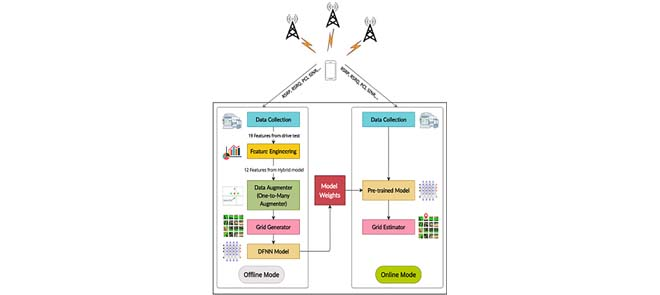
\includegraphics[scale = 2]{images/access-gagraphic-3140292.jpg}
    \caption{DeepFeat system architecture}
    \label{fig:dpft_sys_arch}
\end{figure}

Various \ac{lte} features are collected via intensive drive test in a large-scale area using the Data Collection module during the offline mode.
The DeepFeat model includes a feature selection module, that differs from previously used selection modules.
DeepFeat uses one-to-many data augmenter to extend the number of samples and reduce the noise impact.
Finally, DeepFeat uses a \ac{dfnn} model, and the most influential collected features are used for training this model.
During the online mode, the desired features are collected from the \ac{ue}.
Then, we use the weights of the trained model for the prediction.
The mobile device location is then estimated using the trained model to predict the grid where the mobile device is located.
using The DeepFeat Technique in small-scale area results in median accuracy of 13.179m.
In comparison, the large-scale area results in median accuracy of 13.7m, which indicates that DeepFeat is a robust outdoor localization system even in a large-scale area.
\chapter{Indoor Localization}



\pagenumbering{Alph}
\printacronyms[pages={display=all,seq/use=false}]
\bibliographystyle{plain}
\bibliography{refrences}
\end{document}
